
% ==========================================
%  SYSTEM AUTOPSY DASHBOARD (2x2 Grid)
% ==========================================
\usepackage{tikz}
\usepackage{pgfplots}
\pgfplotsset{compat=1.18}
\definecolor{kafkaBlue}{HTML}{4C72B0} % Muted Academic Blue
\definecolor{lladaRed}{HTML}{C44E52}  % Muted Brick Red

\begin{figure}[p]
    \centering

    % --- CHART A: COGNITIVE TOPOLOGY (Nodes) ---
    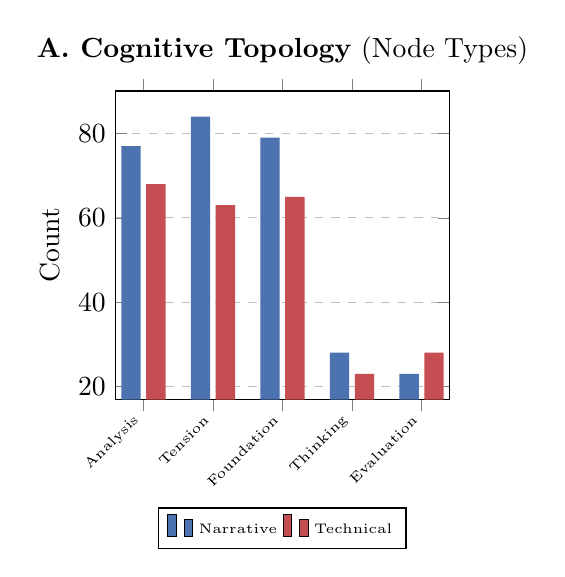
\begin{tikzpicture}
        \begin{axis}[
            ybar, bar width=7pt, width=0.48\linewidth, height=5.5cm,
            title={\textbf{A. Cognitive Topology} (Node Types)},
            ylabel={Count},
            symbolic x coords={Analysis, Tension, Foundation, Thinking, Evaluation},
            xtick=data, x tick label style={rotate=45, anchor=east, font=\tiny},
            nodes near coords style={font=\tiny},
            legend style={at={(0.5,-0.35)}, anchor=north, legend columns=-1, font=\tiny},
            ymajorgrids=true, grid style=dashed
        ]
        % Narrative
        \addplot[fill=kafkaBlue, draw=none] coordinates {
            (Analysis,77) (Tension,84) (Foundation,79) (Thinking,28) (Evaluation,23)
        };
        % Technical
        \addplot[fill=lladaRed, draw=none] coordinates {
            (Analysis,68) (Tension,63) (Foundation,65) (Thinking,23) (Evaluation,28)
        };
        \legend{Narrative, Technical}
        \end{axis}
    \end{tikzpicture}
    \hfill
    % --- CHART B: STRUCTURAL INTEGRITY (Metrics) ---
    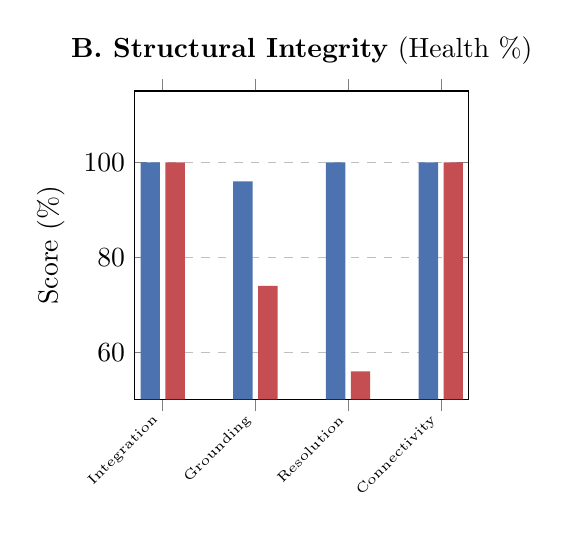
\begin{tikzpicture}
        \begin{axis}[
            ybar, bar width=7pt, width=0.48\linewidth, height=5.5cm,
            title={\textbf{B. Structural Integrity} (Health \%)},
            ylabel={Score (\%)},
            symbolic x coords={Integration, Grounding, Resolution, Connectivity},
            xtick=data, x tick label style={rotate=45, anchor=east, font=\tiny},
            ymax=115, nodes near coords style={font=\tiny},
            legend style={at={(0.5,-0.35)}, anchor=north, legend columns=-1, font=\tiny},
            ymajorgrids=true, grid style=dashed
        ]
        % Narrative
        \addplot[fill=kafkaBlue, draw=none] coordinates {
            (Integration,100) (Grounding,96) (Resolution,100) (Connectivity,100)
        };
        % Technical
        \addplot[fill=lladaRed, draw=none] coordinates {
            (Integration,100) (Grounding,74) (Resolution,56) (Connectivity,100)
        };
        \end{axis}
    \end{tikzpicture}

    \vspace{0.5cm}

    % --- CHART C: RELATIONAL LOGIC (Edge Types) ---
    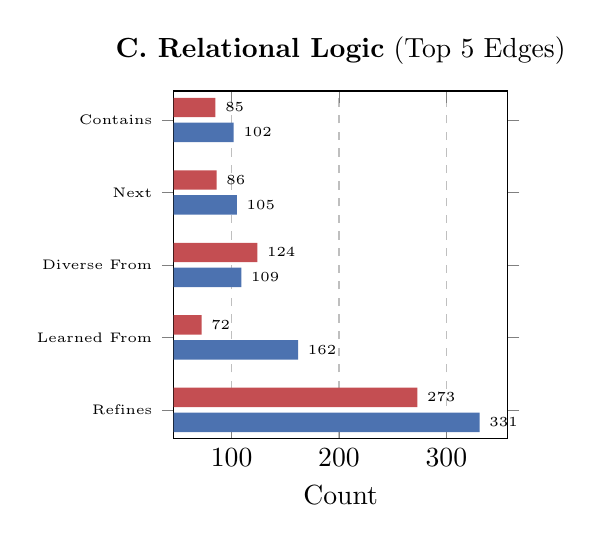
\begin{tikzpicture}
        \begin{axis}[
            xbar, bar width=7pt, width=0.48\linewidth, height=6cm,
            title={\textbf{C. Relational Logic} (Top 5 Edges)},
            xlabel={Count},
            symbolic y coords={Refines, Learned From, Diverse From, Next, Contains},
            ytick=data, y tick label style={font=\tiny},
            nodes near coords, nodes near coords align={horizontal},
            nodes near coords style={font=\tiny, color=black},
            legend style={at={(0.5,-0.25)}, anchor=north, legend columns=-1, font=\tiny},
            xmajorgrids=true, grid style=dashed,
            reverse legend
        ]
        % Narrative
        \addplot[fill=kafkaBlue, draw=none] coordinates {
            (331,Refines) (162,Learned From) (109,Diverse From) (105,Next) (102,Contains)
        };
        % Technical
        \addplot[fill=lladaRed, draw=none] coordinates {
            (273,Refines) (72,Learned From) (124,Diverse From) (86,Next) (85,Contains)
        };
        \end{axis}
    \end{tikzpicture}
    \hfill
    % --- CHART D: STIGMERGIC LABOR (Agents) ---
    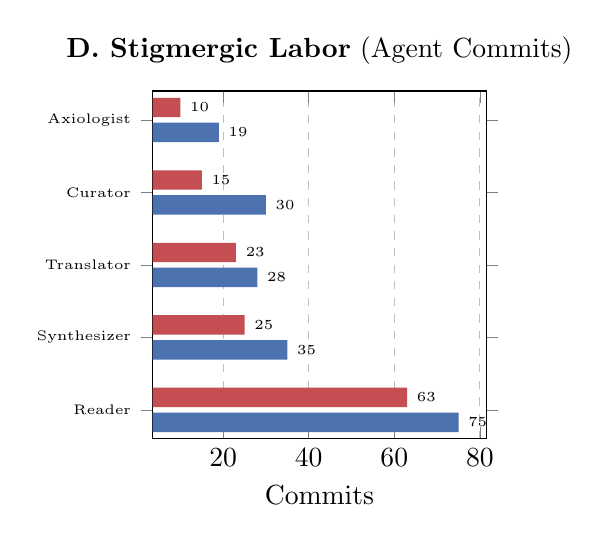
\begin{tikzpicture}
        \begin{axis}[
            xbar, bar width=7pt, width=0.48\linewidth, height=6cm,
            title={\textbf{D. Stigmergic Labor} (Agent Commits)},
            xlabel={Commits},
            symbolic y coords={Reader, Synthesizer, Translator, Curator, Axiologist},
            ytick=data, y tick label style={font=\tiny},
            nodes near coords, nodes near coords align={horizontal},
            nodes near coords style={font=\tiny, color=black},
            legend style={at={(0.5,-0.25)}, anchor=north, legend columns=-1, font=\tiny},
            xmajorgrids=true, grid style=dashed,
            reverse legend
        ]
        % Narrative
        \addplot[fill=kafkaBlue, draw=none] coordinates {
            (75,Reader) (35,Synthesizer) (28,Translator) (30,Curator) (19,Axiologist)
        };
        % Technical
        \addplot[fill=lladaRed, draw=none] coordinates {
            (63,Reader) (25,Synthesizer) (23,Translator) (15,Curator) (10,Axiologist)
        };
        \end{axis}
    \end{tikzpicture}

    \caption{\textbf{System Autopsy.} A comprehensive view of the multi-agent architecture across domains.
    \textbf{(A)} The system prioritizes Tension in narratives vs. Analysis in technical texts.
    \textbf{(B)} Structural integrity (Integration) remains at 100\% across domains.
    \textbf{(C)} The dominance of ``Refines'' proves the system is iterative; note LLaDA's higher ratio of ``Diverse From'' (differentiation) vs. ``Learned From.''
    \textbf{(D)} The division of labor shows the pipeline from Reading (input) to Synthesis/Translation (output), with the Curator working harder on the ambiguous Narrative text.}
    \label{fig:dashboard}
\end{figure}
